\subsubsection{Чем определяется тепловой ток p-n перехода? Какую информацию несёт в себе его значение?}

%Обозначим через $\tau$ неравновесное время жизни избыточных носителей:
%$$
%\tau = \left(\frac{1}{\tau_n} + \frac{1}{\tau_p} \right)^{-1}
%$$
%Причём в условиях нейтральности это время одинаково для электронов и дырок. Очевидно, что $\tau$ %ближе к меньшему из двух равновесных времен жизни. 
Рассмотрим одно из уравнений диффузии:
\begin{equation}
\frac{\partial p}{\partial t} = - \frac{p - p_0}{\tau_p} + D_p\frac{\partial^2p}{\partial x^2}
\end{equation}

Будем считать p-n переход несимметричным и p-слой значительно больше легированным. При этом можно сосредоточить внимание на анализе процессов в базе, а результаты анализа затем распространить на аналогичные, менее существенные процессы в эмиттере.

Рассмотрим статический режим. Получим стационарное распределение дырок в базе. Для этого положим
$$
\frac{\partial \Delta p}{\partial t} = 0
$$

Получим
$$
\frac{\partial^2p}{\partial x^2} - \frac{\Delta p}{L_p^2} = 0
$$

Т.к. $p = p_0 + \Delta p$, 

$$
\frac{\partial^2\Delta p}{\partial x^2} - \frac{\Delta p}{L_p^2} = 0
$$

Решением такого дифференциального уравнения является сумма экспонент:
$$
\Delta p_n = A_1 exp\left(\frac{x}{\sqrt{D_p\tau}}\right) + A_2 exp\left(-\frac{x}{\sqrt{D_p\tau}}\right)
$$

Найдём коэффициенты, воспользовавшись граничными условиями:
$$
\Delta p(0) = p_0\left(e^{\frac{U}{\varphi_T}} - 1\right)
$$

Считая, что на омическом контакте концентрации носителей имеют равновесное значение, запишем
$$
\Delta p(w) = 0
$$, где $w$ - ширина базы.
Для достаточно толстой базы ($w > (2-3)L$ можно положить $w \rightarrow \infty$. Тогда можно записать коэффициенты в следующем виде:
$$
A_1 = 0; A_2 = \Delta p(0)
$$

В этом случае можно записать
$$
\Delta p(x) = p_0 \left(exp\left[\frac{U}{\varphi_T}\right] -1 \right) exp\left[-\frac{x}{L}\right]
$$

Т.к.
$$
j_p = -qD_p\frac{dp}{dx}
$$

В свою очередь, 
$$
I_p = j_p \cdot S = -qD_pS\frac{dp}{dx} 
$$

Тогда 
$$
I_p(x) = \underbrace{\frac{qD_pSp_{n_0}}{L_p}}_{I_0}\left[exp\left(\frac{U}{\varphi_T}\right) -1 \right] exp\left[-\frac{x}{L}\right]
$$
Нас интересует ток через p-n переход. Положим x=0:
\begin{equation}
I = I_0\left(e^{\frac{U}{\varphi_T}} -1 \right)
\end{equation}

Дырочная составляющая тока является основной, поэтому $I_n$ можно пренебречь и дать определению тепловому току $I_0$ как это сделано выше.

Тепловой ток $I_0$ определяет масштаб ВАХ. Термин "тепловой" отражает сильную температурную зависимость этого тока. Также он равен 0 при абсолютном нуле температуры. Также его называют обратным током насыщения, что связано с тем, что при обратном смещении обратный ток идеализированного диода равен $-I_0$ и не зависит от напряжения.

\begin{center}
	\begin{figure}[h!]
		\center{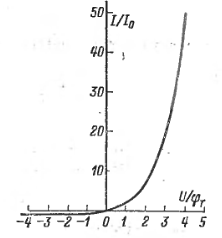
\includegraphics[scale=1]{VAH.png}}
		\caption{ВАХ p-n перехода}
	\end{figure}
\end{center}


